% Presentation draft. No invented learner, provider or final billing results.
% Use installed Tectonic with --only-cached. All graphics are local/public.
\documentclass[12pt]{article}
\usepackage[paperwidth=320mm,paperheight=180mm,margin=12mm]{geometry}
\usepackage{lmodern,fontspec}
\setmainfont{Arial}[BoldFont={Arial Bold},ItalicFont={Arial Italic},BoldItalicFont={Arial Bold Italic}]
\setsansfont{Arial}[BoldFont={Arial Bold},ItalicFont={Arial Italic},BoldItalicFont={Arial Bold Italic}]
\setmonofont{Menlo}
\usepackage{graphicx,tabularx,array,booktabs}
% Tables use an invisible math strut. Reuse the report's cached math size.
\DeclareMathSizes{18}{11}{8}{6}
\DeclareMathSizes{13}{11}{8}{6}
\DeclareMathSizes{12}{11}{8}{6}
\usepackage{tikz}
\usetikzlibrary{arrows.meta}
\pgfdeclarelayer{shadow}
\pgfsetlayers{shadow,main}
\usepackage[hidelinks]{hyperref}
\usepackage{xurl}
\definecolor{Ink}{HTML}{171717}
\definecolor{Paper}{HTML}{FAF7EE}
\definecolor{Signal}{HTML}{FFD335}
\definecolor{Blue}{HTML}{B7D7FF}
\definecolor{Pink}{HTML}{F2B9D2}
\pagecolor{Paper}
\color{Ink}
\renewcommand{\familydefault}{\sfdefault}
\setlength{\parindent}{0pt}
\setlength{\parskip}{4mm}
\setlength{\emergencystretch}{1em}
\raggedright
\newcolumntype{Y}{>{\raggedright\arraybackslash}X}
\pagestyle{empty}
\newcommand{\Slide}[3]{%
 \clearpage
 \begin{tikzpicture}[remember picture,overlay]
 \draw[line width=1.3pt] ([xshift=12mm,yshift=12mm]current page.south west)
   -- ([xshift=-12mm,yshift=12mm]current page.south east);
 \node[anchor=south west,font=\fontsize{10}{12}\selectfont]
   at ([xshift=12mm,yshift=4.5mm]current page.south west)
   {OPSREPLAY / CS5224 GROUP 26 / WORKING DRAFT 1 NOV 2026};
 \node[anchor=south east,font=\fontsize{10}{12}\selectfont]
   at ([xshift=-12mm,yshift=4.5mm]current page.south east)
   {#3\quad\textbar\quad\thepage};
 \end{tikzpicture}\par
 {\fontsize{12}{14}\selectfont\bfseries #1\par}
 \vspace{1mm}
 {\fontsize{32}{36}\selectfont\bfseries #2\par}
 \vspace{3mm}
 \fontsize{18}{23}\selectfont
}
\newcommand{\Panel}[3]{%
 \begin{tikzpicture}
 \node[draw=Ink,line width=1.1pt,fill=#2,text width=\dimexpr#1-8mm\relax,
   inner sep=4mm,align=left,anchor=center] (panel) at (0,0) {#3};
 \begin{pgfonlayer}{shadow}
 \fill[Ink] ([xshift=1mm,yshift=-1mm]panel.south west)
   rectangle ([xshift=1mm,yshift=-1mm]panel.north east);
 \end{pgfonlayer}
 \end{tikzpicture}\par
}
\newcommand{\Small}{\par\fontsize{13}{17}\selectfont}
\newcommand{\Evidence}[1]{\par\smallskip{\fontsize{11}{14}\selectfont\color{Ink!80}#1\par}}
\hypersetup{pdftitle={OpsReplay CS5224 Presentation Working Draft},pdfauthor={CS5224 Group 26}}

\begin{document}
\Slide{01 / PRODUCT}{Learn production failures by investigating them.}{BLOCK A / 00:00--00:20}
\vspace{4mm}
{\fontsize{58}{62}\selectfont\bfseries OpsReplay\par}
\vspace{3mm}
\Panel{282mm}{Signal}{Real services. Evidence. Recovery. Debrief. Playback.}
\vspace{3mm}
\Small
Lee Hao Zhe / Neeraj Kumbar / Neo Qi Hao / Poh Yu Wen / See Yang Zhi / Teo Kai Xiang
\par
\Evidence{Implemented source: 5c33055. Draft results have explicit environment and revision limits.}

\Slide{01 / PROBLEM}{The first production incident is a poor classroom.}{BLOCK A / 00:20--01:00}
\begin{minipage}[t]{0.47\linewidth}
\vspace{0pt}\raggedright
\textbf{Who needs practice?}\par
CS and cloud students.\par
Junior software, DevOps and SRE engineers.
\end{minipage}\hfill
\begin{minipage}[t]{0.47\linewidth}
\vspace{0pt}\raggedright
\textbf{What reading cannot test}\par
Which signal matters?\par
What evidence supports the cause?\par
Will this intervention help or harm?
\end{minipage}\par
\vspace{7mm}
\Panel{282mm}{Blue}{A learner must investigate incomplete evidence and assess the actual result.}
\Evidence{Educational reference: Google SRE Wheel of Misfortune. Learning benefit remains to be evaluated.}

\Slide{01 / MECHANISM}{One investigation, followed by evidence-based feedback.}{BLOCK A / 01:00--01:30}
\vspace{4mm}
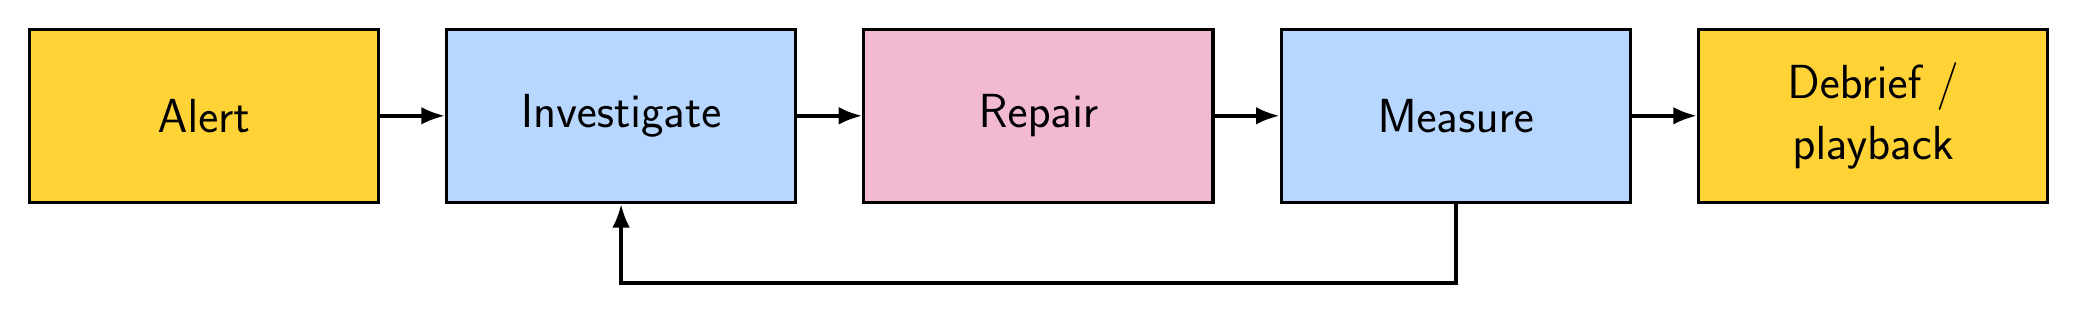
\begin{tikzpicture}[n/.style={draw,line width=1.1pt,fill=Signal,align=center,
 text width=42mm,minimum height=22mm,font=\fontsize{18}{22}\selectfont},
 a/.style={-{Latex[length=3mm]},line width=1.4pt}]
\node[n] (alert) at (0,0) {Alert};
\node[n,fill=Blue] (inspect) at (5.3,0) {Investigate};
\node[n,fill=Pink] (repair) at (10.6,0) {Repair};
\node[n,fill=Blue] (measure) at (15.9,0) {Measure};
\node[n] (review) at (21.2,0) {Debrief /\\playback};
\draw[a] (alert) -- (inspect);
\draw[a] (inspect) -- (repair);
\draw[a] (repair) -- (measure);
\draw[a] (measure) -- (review);
\draw[a] (measure.south) -- ++(0,-1) -| (inspect.south);
\end{tikzpicture}\par
\vspace{7mm}
Real terminal and telemetry. Any valid repair can work.\par
External checks confirm sustained recovery. A retry creates a fresh task.
\Evidence{Existing products include SadServers and SimIncident. OpsReplay's integrated workflow is a positioning hypothesis.}

\Slide{02 / OFFER}{A complete Free sample. Additional practice in Pro.}{BLOCK B / 01:30--02:15}
\begin{minipage}[t]{0.46\linewidth}
\vspace{0pt}\raggedright
\Panel{132mm}{Blue}{\textbf{Free}\par
Introductory content in each mode.\par
Full Challenge debrief, playback and fresh retries.}
\end{minipage}\hfill
\begin{minipage}[t]{0.46\linewidth}
\vspace{0pt}\raggedright
\Panel{132mm}{Signal}{\textbf{Pro: proposed S\$12/month}\par
Expanded published content.\par
Longer Challenge sessions.}
\end{minipage}\par
\vspace{7mm}
\textbf{Demo upgrade:} fixed-window, server-owned grant.\par
No payment, recurring charge or automatic renewal.
\Evidence{Current library: 2 Challenges, 2 lessons and 1 published Code Review. Institutional seats are future work.}

\Slide{02 / ECONOMICS}{Revenue must cover delivery and content operations.}{BLOCK B / 02:15--03:00}
\Panel{282mm}{Signal}{\textbf{S\$12 revenue − S\$1.82 delivery − S\$0.99 future fees = S\$9.19 contribution}}
\vspace{4mm}
\begin{minipage}[t]{0.48\linewidth}
\vspace{0pt}\raggedright
\textbf{Working monthly assumptions}\par
6 paid Challenge hours per subscriber.\par
5 active Free learners per subscriber.\par
S\$972.07 fixed operating allocation.
\end{minipage}\hfill
\begin{minipage}[t]{0.46\linewidth}
\vspace{0pt}\raggedright
\textbf{Operating break-even}\par
{\fontsize{43}{46}\selectfont\bfseries 106 subscribers\par}
\Small
At 60 paid hours: 208 subscribers.\par
Usage and willingness to pay are unvalidated.
\end{minipage}\par
\Evidence{Pricing proposal, 26 October. FX S\$1.35/US\$1. Excludes engineering payroll, startup recovery and tax. Fees are future assumptions.}

\Slide{03 / ARCHITECTURE}{Managed control plane. Private per-attempt compute.}{BLOCK C / 03:00--04:05}
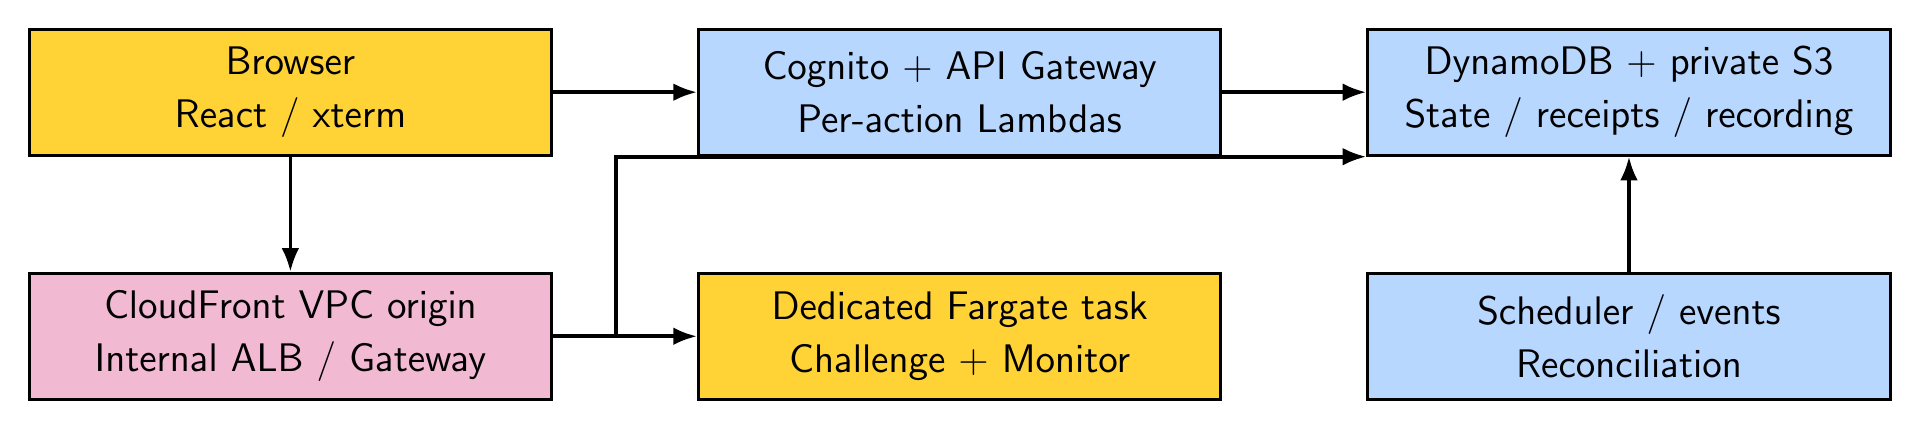
\begin{tikzpicture}[n/.style={draw,line width=1.1pt,fill=Blue,align=center,
 minimum height=16mm,text width=64mm,font=\fontsize{15}{19}\selectfont},
 a/.style={-{Latex[length=3mm]},line width=1.3pt}]
\node[n,fill=Signal] (browser) at (0,0) {Browser\\React / xterm};
\node[n] (api) at (8.5,0) {Cognito + API Gateway\\Per-action Lambdas};
\node[n] (store) at (17,0) {DynamoDB + private S3\\State / receipts / recording};
\node[n,fill=Pink] (gateway) at (0,-3.1) {CloudFront VPC origin\\Internal ALB / Gateway};
\node[n,fill=Signal] (attempt) at (8.5,-3.1) {Dedicated Fargate task\\Challenge + Monitor};
\node[n] (lifecycle) at (17,-3.1) {Scheduler / events\\Reconciliation};
\draw[a] (browser) -- (api);
\draw[a] (api) -- (store);
\draw[a] (browser) -- (gateway);
\draw[a] (gateway) -- (attempt);
\draw[a] (gateway.east) -- ++(0.8,0) |- (store.south west);
\draw[a] (lifecycle) -- (store);
\end{tikzpicture}\par
\vspace{2mm}
\Small
Static SPA: private S3 + CloudFront. Each Lambda has its own role and limits.\par
Challenge: no task IAM role and no internet route. The Gateway owns recording.
\Evidence{Architecture and bounded AWS qualification at merged source 5c33055. Runtime is removed after the campaign.}

\Slide{03 / RELIABILITY}{One request identity. One attempt. One saved result.}{BLOCK C / 04:05--05:00}
\begin{minipage}[t]{0.48\linewidth}
\vspace{0pt}\raggedright
\textbf{Before launch}\par
Validate owner, content and access.\par
Atomically save receipt, session, lock and launch arguments.\par
Recover the same request after response loss.
\end{minipage}\hfill
\begin{minipage}[t]{0.46\linewidth}
\vspace{0pt}\raggedright
\textbf{Before result publication}\par
Fix one outcome and recording cutoff.\par
Drain recording; confirm task stop.\par
Commit debrief and release the matching lock.
\end{minipage}\par
\vspace{5mm}
\Panel{282mm}{Pink}{Incomplete recording has no numeric score. A retry preserves the first attempt.}
\Evidence{1 November: lost/duplicate start, active end, token expiry, reconnect and controlled Gateway replacement passed. Larger recovery capacity is unmeasured.}

\Slide{04 / CHALLENGE DEMO}{Investigate. Repair. Observe recovery.}{BLOCK D / 05:00--09:00}
\begin{minipage}[t]{0.48\linewidth}
\vspace{0pt}\raggedright
\textbf{Show the actual application}\par
1. Briefing and owned attempt.\par
2. Logs, listeners and configuration.\par
3. A validated repair.\par
4. Sustained recovery.\par
5. Debrief and synchronized playback.
\end{minipage}\hfill
\begin{minipage}[t]{0.46\linewidth}
\vspace{0pt}\raggedright
\Panel{132mm}{Signal}{\textbf{60 seconds}\par
The reference validator requires continued service recovery.}
\vspace{4mm}
\Small
Explain admission during provisioning.\par
Explain measured impact during recovery.\par
Navigation does not pause the incident.
\end{minipage}\par
\Evidence{Rehearsal pending. Live use requires an approved runtime window. A fallback must be labelled recorded, with revision and date.}

\Slide{05 / CODE REVIEW}{Flag a risky line. Keep the reasoning. Review the result.}{BLOCK E / 09:00--10:15}
\begin{minipage}[t]{0.48\linewidth}
\vspace{0pt}\raggedright
\textbf{Learner interaction}\par
Keyboard line selection.\par
Inline concerns with edit/delete.\par
Version-bound draft survives refresh.\par
Saved result reopens from History.
\end{minipage}\hfill
\begin{minipage}[t]{0.46\linewidth}
\vspace{0pt}\raggedright
\Panel{132mm}{Blue}{\textbf{Feedback boundary}\par
Line matching is deterministic.\par
Written concerns are not graded.}
\vspace{4mm}
\Small
Learn links incident explanations to practice.\par
Show temporary Pro access without payment.
\end{minipage}\par
\Evidence{29 October: review editing, refresh, submission POST response loss and saved-result recovery passed.}

\Slide{05 / OPTIONAL ASSISTANT}{Explain evidence. Propose a command. Wait for confirmation.}{BLOCK E / 10:15--11:00}
\Panel{282mm}{Pink}{\textbf{Learner question / public context / typed proposal / explicit confirmation}}
\vspace{4mm}
The backend owns evidence, outcomes and scoring.\par
Unknown dispatch is not automatically resent.\par
The terminal and investigation remain usable when the provider fails.
\vspace{3mm}
\Small
19 baseline attempts: 18 complete, 1 failed. Adapter p50 / p95: 4.62 / 6.01 s.\par
Two deployed streams: 8.57 / 6.64 s. Repeated confirmation counted once.
\Evidence{Manual rubric: 4/18 replies had unsupported facts. PR \#137 narrows instructions. Small sample; no accuracy guarantee or enforced billing cap.}

\Slide{06 / SYSTEM RESULTS}{450 owned GETs passed. Capacity is still unmeasured.}{BLOCK F / 11:00--11:50}
\begin{center}
\renewcommand{\arraystretch}{1.4}
\begin{tabularx}{0.94\linewidth}{@{}Yrr@{}}
\toprule
Endpoint & 1 worker p50 / p95 (ms) & 2 workers p50 / p95 (ms)\\
\midrule
Catalogue & 75 / 249 & 60 / 231\\
Account & 66 / 221 & 54 / 219\\
Session & 71 / 190 & 48 / 208\\
\bottomrule
\end{tabularx}
\end{center}
\vspace{2mm}
2-second think time. 1.33 / 2.68 requests per second for this mix.\par
No task start, terminal ticket, presence refresh or session mutation.
\Evidence{29 October AWS checkpoint, source e59067b. One Gateway and two serial Challenge attempts. No classroom or paid-capacity claim.}

\Slide{06 / HOSTING COST}{Idle services and operator time affect the result.}{BLOCK F / 11:50--12:55}
\begin{center}
\renewcommand{\arraystretch}{1.3}
\begin{tabularx}{0.94\linewidth}{@{}Yrr@{}}
\toprule
Challenge hours/month & Cloud projection (S\$) & On-premise working case (S\$)\\
\midrule
50 & 236.23 & 470.33\\
400 & 265.34 & 470.33\\
1200 & 331.89 & 470.33\\
\bottomrule
\end{tabularx}
\end{center}
\Small
Assume S\$4,000 host / 36 months, 100 W, S\$0.2859/kWh and 1.4 power overhead.\par
Cloud: 2 operating hours/month. On-premise: 6 hours + amortised adapter work.\par
Equal labour and no new adapter work: on-premise falls to S\$300.33/month.
\Evidence{Sensitivity only. Capacity, power, labour, final charges and equivalent availability remain unverified. Equal provider/content costs excluded.}

\Slide{06 / LEARNER EVALUATION}{Test reasoning and usability with real learners.}{BLOCK F / 12:55--13:45}
\begin{minipage}[t]{0.48\linewidth}
\vspace{0pt}\raggedright
\textbf{Prepared protocol}\par
5--10 students or junior engineers.\par
One interactive incident; one static case.\par
Counterbalanced order; assistant off.\par
Baseline, post and transfer questions; SUS.
\end{minipage}\hfill
\begin{minipage}[t]{0.46\linewidth}
\vspace{0pt}\raggedright
\Panel{132mm}{Blue}{\textbf{Results: not collected}\par
No learning-effectiveness or retention claim.}
\vspace{4mm}
\Small
The two incidents differ in difficulty.\par
Report by incident and condition.\par
Missing results stay missing.
\end{minipage}\par
\Evidence{Ten synthetic fixtures checked score calculations only; no person participated. Real testing needs a study contact, consent and deletion date.}

\Slide{06 / READINESS}{The main learner loop works. Final gates remain open.}{BLOCK F / 13:45--14:30}
\begin{minipage}[t]{0.48\linewidth}
\vspace{0pt}\raggedright
\Panel{132mm}{Signal}{\textbf{Verified}\par
Email sign-up and access checks.\par
Both real Challenge recovery paths.\par
Debrief, playback and temporary cleanup.\par
Current frontend and component checks.}
\end{minipage}\hfill
\begin{minipage}[t]{0.46\linewidth}
\vspace{0pt}\raggedright
\Panel{132mm}{Pink}{\textbf{Still required}\par
Participant study and outcomes.\par
Residual image-finding assessment.\par
Host capacity and cost evidence.\par
Final attributed charges and rehearsal.}
\end{minipage}\par
\Evidence{1 November exact-image scans: Gateway/Monitor reported no findings; each Challenge had 1 HIGH, 3 MEDIUM, 3 LOW. Three named glibc findings have scoped owner acceptance.}

\Slide{06 / DELIVERY}{Practice the failure. Learn from the recorded path.}{BLOCK F / 14:30--15:00}
\vspace{4mm}
\Panel{282mm}{Signal}{\textbf{OpsReplay}\par
Real-service investigation, independent recovery checks and structured feedback.}
\vspace{4mm}
\textbf{Public code}\par
\url{https://github.com/ehz0ah/OpsReplay}
\vspace{3mm}
\Small
AI assisted code, tests, UI refinements, review fixes and this draft.\par
The team must verify the disclosure and add its own learning statement.
\Evidence{Draft is not submission-ready. Required outcomes and the team's final learning statement remain incomplete.}

\Slide{BACKUP / OPERATIONS}{Admission, recording and erasure have distinct checks.}{Q\&A BACKUP / NOT TIMED}
One active attempt per learner; current access is server-validated.\par
Recording generations fence stale writers. First outcome fixes the cutoff.\par
Independent Monitor data determines recovery and raw impact components.\par
Operator-only erasure waits 120 seconds after a saved marker, then verifies\par
object-prefix, session-partition and owner-reference absence.
\Evidence{1 November AWS erasure passed: pending, deleted, absent on replay; unrelated rows preserved. This is one-session deletion, not account or backup erasure.}

\Slide{BACKUP / CODE}{Separate action handlers. Shared ordinary modules.}{Q\&A BACKUP / NOT TIMED}
\Small
\renewcommand{\arraystretch}{1.35}
\begin{tabularx}{\linewidth}{@{}p{66mm}Y@{}}
\toprule
\texttt{apps/web} & Learner routes, identity, terminal, review drafts and playback\\
\texttt{apps/api} & Per-action ownership, admission, reads, writes and assistant\\
\texttt{apps/gateway} & Terminal generations, recording and proposal delivery\\
\texttt{apps/monitor} & External probes, metrics and sustained recovery\\
\texttt{packages/session} & Lifecycle, evidence derivation and once-only finalisation\\
\texttt{content / contracts} & Authored versions, restricted projections and wire schemas\\
\texttt{infra / scripts} & CDK deployment/cleanup and explicit evaluation tools\\
\bottomrule
\end{tabularx}
\vspace{4mm}
\Evidence{One deployed Lambda per action. No Lambda-to-Lambda invocation. Local checks do not establish managed AWS behaviour.}

\Slide{BACKUP / REFERENCES}{Source records and working assumptions}{Q\&A BACKUP / NOT TIMED}
\Small
\setlength{\parskip}{2.5mm}
\textbf{Product and training references}\par
Google SRE: \url{https://sre.google/workbook/postmortem-culture/}\par
SadServers: \url{https://sadservers.com/faq}\quad
SimIncident: \url{https://simincident.com/}\par
\textbf{OpsReplay evidence at source 5c33055}\par
\texttt{docs/checkpoints/2026-10-29-saas-aws.md}\par
\texttt{docs/checkpoints/2026-11-01-release-qualification.md}\par
\texttt{docs/decisions/pricing-proposal.md}\par
\texttt{docs/decisions/neobrutalist-discovery.md}\par
\texttt{docs/evaluation/pilot/README.md}\par
\textbf{Cost sources}\par
SP Group Q4 tariff; dated AWS Singapore rates; Stripe Singapore pricing.\par
Full URLs, configuration limits and assumptions are in the report and\par
\texttt{docs/reports/final/cost-comparison.md}.
\end{document}
